\section{Tia Nur Candida (1174086)}
\subsection{Buku}
Rp.100.000(Lunas)
\subsection{Pengertian}
	Sistem Informasi Geografis diartikan sebagai sistem untuk menyimpan, memeriksa, mengintegrasi, memanipulasi, menganalisis, dan memaparkan data yang berkaitan dengan semua ruang yang berhubungan dengan bumi. 

\subsection{Sejarah}
	Peta merupakan penggambaran sejarah secara grafis atau bentuk skala pada konsep mengenai bumi dalam hal ini peta merupakan alat untuk menyampaikan atau menginformasikan mengenai ilmu kebumian peta. Menurut Claudius ptolemy Claudius ptolomeus yang dikenal dengan nama polemik ptolemy hidup antara tahun 100 m dan 168 m beliau merupakan salah satu sarjana sains pada masanya dia tinggal dan bekerja di Alexandria di kota Mesir yang merupakan pusat intelektual dunia barat dengan perpustakaan paling luas yang pernah diciptakan ptolemy membawa semua pengetahuan dan keterampilan matematika dan astronomi dan menerapkannya pada pembuatan peta, Dia memiliki daya tarik matematikawan dengan presisi untuk menunjukkan hubungan satu tempat ke tempat lain berdasarkan perhitungan lingkaran dunia 18000 mil Ia juga mengembangkan sistem Grid latitude dan longitude yang dirancang oleh marinus of the fire sementara beberapa rincian peta Mungkin sedikit aneh dengan garis lintang yang sejajar dengan garis Khatulistiwa dengan garis bujur yang membentang ke utara selatan dengan busur Anggun sudah tidak asing lagi bagi siapa saja yang pernah memiliki Atlas ptolemy mampu membangun koordinat dan mendaftarkan lebih dari 8000 tempat dengan koordinat masing-masing 
data-data tentang pembuatan peta sempat hilang ketika perpustakaan Alexandria yang terkenal dibakar oleh orang-orang Kristen fanatik pada tahun 390 masehi sebuah contoh awal konflik antara iman dan sains tetapi satu salinan yang telah dibuat dari karya ptolemy terselamatkan dan bertahan di byzantium

\subsection{Koordinat}
	Sistem koordinat dimaksudkan untuk memberikan pengalamatan terhadap setiap lokasi di permukaan bumi dimana pengalamatan dengan sistem koordinat didasarkan pada jarak Timur Barat dan Utara Selatan suatu tempat dari suatu titik pangkal tertentu jarak diukur dalam satuan derajat sudut yang dibentuk dari titik pangkal ke posisi tersebut melalui pusat bumi sedangkan titik pangkal ditetapkan berada di perpotongan belahan utara selatan bumi atau garis Khatulistiwa dengan garis yang membelah bumi Timur Barat koordinat diambil untuk menjadi bilangan riil dalam matematika dasar tetapi memungkinkan bilangan kompleks atau elemen dari sistem yang lebih abstrak penggunaan sistem koordinat memungkinkan masalah dalam angka untuk diterjemahkan kedalam masalah-masalah tentang geometri dan juga sebaliknya.
	Garis lintang dapat disebut juga sebagai garis khatulistiwa 0 derajat atau bisa disebut juga sebagai garis tengah bumi yang membagi antara belahan bumi bagian atas dan bumi bagian bawah garis lintang digunakan sebagai penanda dalam zona iklim di dunia dari + 23 setengah derajat lintang utara sampai Min 23 setengah Lintang Selatan memiliki zona iklim tropis zona iklim tropis hanya memiliki dua musim yaitu kemarau atau panas dan penghujan saja Kemudian dari + 23 setengah derajat lintang utara sampai dengan + 66 setengah derajat Lintang Utara memiliki zona iklim subtropis Sama halnya bagian utara bagian Selatan yaitu Min 23 setengah derajat Lintang Selatan sampai 66 setengah derajat Lintang Selatan memiliki zona iklim subtropis daerah subtropis memiliki 4 musim yaitu spring Summer fall and winter. garis bujur bisa digunakan untuk menentukan waktu dan tanggal di dunia yang kita huni sekarang Jika garis lintang atau Latitude atau daerah khatulistiwa dianggap sebagai 0 derajat maka garis bujur merupakan 0 derajat yang menghubungkan Kutub Utara dengan kutub selatan yang melewati kota Greenwich di Inggris garis bujur bagian Barat kota Greenwich disebut sebagai bujur barat sedangkan garis bujur yang berada di sebelah timur kota Greenwich disebut sebagai bujur timur

\subsection{Geospasial}
	Informasi geospasial yang biasanya dikenal dengan Peta adalah informasi objek permukaan bumi yang mencakup aspek waktu dan keruangan pengertian gaya dalam geospasial berarti geosfer yang mencakup atmosfer lapisan udara yang meliputi permukaan bumi litosfer lapisan kulit bumi pedosfer tanah beserta pembentukan dan zona-zona nya sebagai bagian dari kulit bumi litosfer lapisan air yang menutupi permukaan bumi dalam berbagai bentuknya biosfer segenap unsur di permukaan bumi yang membuat kehidupan dan proses biotik berlangsung dan antroposfer manusia dengan segala aktivitas yang dilakukannya di permukaan bumi.


\subsection{Link}
https://www.youtube.com/watch?v=zrXFgPf4fLs
\subsection{Plagiarism}
\begin{figure}[H]
	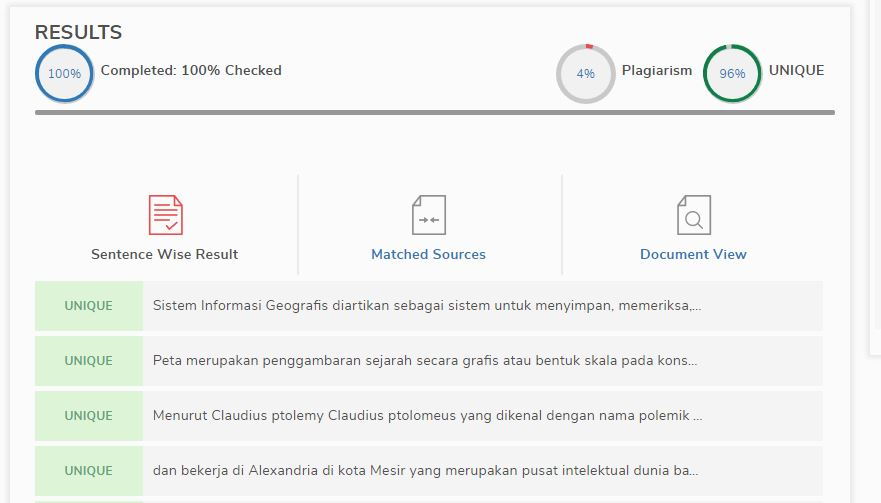
\includegraphics[width=4cm]{figures/Tugas1/1174086/plagiat.jpg}
	\centering
	\caption{Gambar Plagiat}
\end{figure}